\scanpage{16}
et par suite $\Sigma_2^-\cup\Sigma_{\deleted{\unsure{2}}1}^+$ \deleted{\unsure{sera|sont}} est un ouvert connexe de $X$ donc de $X\setminus E_2$,
% Local insertion drawing. Full-scan origin (1045,140); x right, y down;
% both coordinate units 0.014 cm. The declared drawing rectangle does not
% prescribe the typeset word extents. G01 is the bent guide below la comp. conn.
% G02a1/G02a2, G02b and G02c are the four observed right-note path components.
\figure{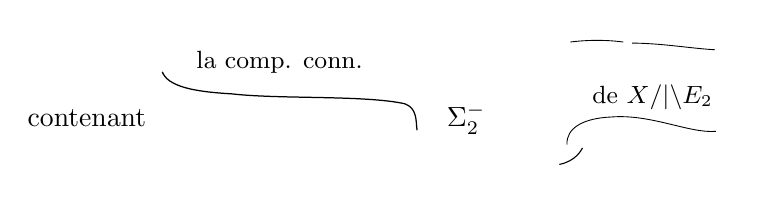
\begin{tikzpicture}[x=0.014cm,y=-0.014cm,baseline={(0,0)}]
  \path[use as bounding box] (0,0) rectangle (640,130);
  \node[anchor=base west,inner sep=0pt,outer sep=0pt] at (0,90) {contenant};
  \node[anchor=base west,inner sep=0pt,outer sep=0pt,font=\small] at (153,37) {\inserted{la comp. conn.}};
  \node[anchor=base west,inner sep=0pt,outer sep=0pt] at (380,90) {$\Sigma_2^-$};
  \node[anchor=base west,inner sep=0pt,outer sep=0pt,font=\small] at (512,69) {\inserted{de $X\unsure{/|\setminus}E_{\unsure{2}}$}};
  % G01: full-scan locus (1165,174)--(1401,236).
  \draw[line width=0.45pt] (122,40) .. controls (127,53) and (149,58) .. (185,60)
    .. controls (228,65) and (306,61) .. (342,69)
    .. controls (353,73) and (352,84) .. (353,93);
  % G02a1 and G02a2: separated portions of the upper rule.
  \draw[line width=0.32pt] (492,13) .. controls (508,11) and (525,11) .. (540,13);
  \draw[line width=0.32pt] (548,14) .. controls (574,14) and (603,19) .. (623,20);
  % G02b: curved lower rule; its continuation reaches the physical right edge.
  \draw[line width=0.32pt] (489,106) .. controls (488,91) and (504,82) .. (529,81)
    .. controls (565,78) and (600,96) .. (624,94);
  % G02c: detached short return below the lower rule.
  \draw[line width=0.4pt] (482,124) .. controls (497,121) and (502,111) .. (503,109);
\end{tikzpicture}}
donc \deleted{\unsure{c'est}} \unsure{égal|égale} \unsure{:|à} $\Sigma_2^-$, \unsure{donc|d'où} $\Sigma_1^+\subset\Sigma_2^-$, \unsure{qfd|cqfd}

L'intersection des deux partitions
\[
 \begin{aligned}
 X&=\deleted{\unsure{E}}\Sigma_1^+\amalg E_1\amalg\Sigma_1^-\\
 X&=\Sigma_2^+\amalg E_2\amalg\Sigma_2^-
 \end{aligned}
\]
de $X$ est
\[
 X=\overbrace{\Sigma_1^+\amalg E_1\amalg
 \rlap{$\displaystyle\underbrace{\phantom{E\Sigma_{12}}\amalg
 E_2\amalg\Sigma_2^+}_{\Sigma_1^-}$}\deleted{E}\Sigma_{12}}^{\Sigma_2^-}
 \phantom{\amalg E_2\amalg\Sigma_2^+}
\]
% M01: small round point at full-scan (429.5,1128.5), below/right of avec.
% The underset is solely a placement device. Hand, surface origin and role remain unresolved.
$\underset{\hspace{2.5em}\unsure{\cdot}}{\text{avec}}$
\[
 \Sigma_{12}\overset{\text{def}}{=}\Sigma_1^-\cap\Sigma_2^-
\]

\deleted{\unsure{O}}Dans cette partition, $\Sigma_1^+,\Sigma_{12},\Sigma_2^+$ sont ouverts $E_1,E_2$ sont fermés, et on a
\[
 \begin{aligned}
 &\Sigma_1^+\subsetneq\overline{\Sigma_1^+}\subset\Sigma_1^+\cup E_1\\
 &\overline{\Sigma_{12}}\subset\overline{\Sigma_1^-}\cap\overline{\Sigma_2^-}\subset
 (\Sigma_1^-\cup E_1)\cap(\Sigma_2^-\cup E_2)\subset\Sigma_{12}\cup E_1\cup E_2\\
 &\Sigma_2^+\subsetneq\overline{\Sigma_2^+}\subset\Sigma_2^+\cup E_2
 \end{aligned}
\]
% M02: two detached points at the right, alongside the last closure row.
% Full-scan local origin (1617,1727), x right, y down, both units 0.018 cm.
% Supported visible point shapes only; hand, surface origin and role unresolved.
\figure{\makebox[\linewidth][r]{\unsure{\begin{tikzpicture}[x=0.018cm,y=-0.018cm,baseline={(0,0)}]
  \path[use as bounding box] (0,0) rectangle (12,16);
  % M02a: upper point, full-scan centre (1625.5,1730.5).
  \fill (8.5,1.9) .. controls (9.3,1.9) and (9.9,2.6) .. (9.9,3.5)
    .. controls (9.9,4.4) and (9.3,5.1) .. (8.5,5.1)
    .. controls (7.7,5.1) and (7.1,4.4) .. (7.1,3.5)
    .. controls (7.1,2.6) and (7.7,1.9) .. (8.5,1.9) -- cycle;
  % M02b: lower point, full-scan reference position (1620.8,1737.5).
  \fill (3.8,10.5) .. controls (4.9,9.4) and (5.5,10.3) .. (5.6,11.3)
    .. controls (4.8,12.1) and (3.4,12.2) .. (2.8,11.8)
    .. controls (2.4,11.1) and (2.9,10.5) .. (3.8,10.5) -- cycle;
\end{tikzpicture}}}}

Notons aussi que
\[
 \overline{\Sigma_{12}}\cap E_1\ne\varnothing,\quad
 % M03: detached point at full-scan (929,1894), above/right of the second cap.
 % The overset preserves position only; no role or hand is assigned.
 \overline{\Sigma_{12}}\overset{\hspace{0.35em}\unsure{\cdot}}{\cap}E_2\ne\varnothing
\]
Car si on avait p.\,ex. $\overline{\deleted{\unsure{E}}\Sigma_{12}}\cap
\deleted{\unsure{\Sigma}}E_1=\varnothing$, on
% G03: cancellation with the inserted wording above it.
% Full-scan drawing origin (300,2194), x right, y down, both units 0.008 cm.
% The phantom preserves the deletion annotation without adding an extra rule.
\figure{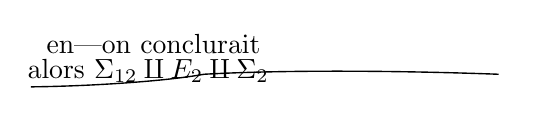
\begin{tikzpicture}[x=0.008cm,y=-0.008cm,baseline={(0,0)}]
  \path[use as bounding box] (0,-80) rectangle (760,25);
  \node[anchor=base west,inner sep=0pt,outer sep=0pt] at (0,0)
    {\rlap{alors $\Sigma_{12}\amalg E_2\amalg\Sigma_2$}\phantom{\deleted{alors $\Sigma_{12}\amalg E_2\amalg\Sigma_2$}}};
  \node[anchor=base west,inner sep=0pt,outer sep=0pt] at (30,-39)
    {\inserted{\unsure{en|on} conclurait}};
  \draw[line width=0.5pt] (5,14) .. controls (100,13) and (220,5) .. (280,-6)
    .. controls (405,-13) and (587,-12) .. (748,-6);
\end{tikzpicture}}
$\overline{\Sigma_1^-}\cap E_1=\varnothing$,
\[
 \begin{aligned}
 \big[\,\text{car}\quad\overline{\Sigma_1^-}&=
 \overline{\Sigma_2^+\deleted{\amalg}\cup E_2
 \deleted{\amalg}\cup\Sigma_{12}}=
 \underbrace{\overline{\Sigma_2^+}}_{\subset\,\Sigma_2^+\cup E_2}\cup E_2
 \cup\overline{\Sigma_{12}}\subset\Sigma_1^-\cup\overline{\Sigma_{12}}\unsure{\big]}
 \end{aligned}
\]
ce qui n'est pas.

% archive sheet number: 15
